% #################################################
% Welcome to the LaTeX template file of Computer-Aided Design and Applications! 
% Please follow the instructions in this document to write and format your paper.
% We appreciate your submission. If you have any question, please feel free to 
% contact us at http://www.cadanda.com/Contactus.html.
% #################################################
\documentclass[9pt,academicons]{article}
\usepackage{SP}
% ####################################
% Add the title of your paper here. Each word is Capitalized! 
% ####################################
\title{Digitale Vernetzung von Sammlungsdaten}
% #################################################
% This is where your paper begins. 
% #################################################
\begin{document}
% #################################################
% Sets up the beginning of the document (do not modify) 
% #################################################
\maketitle
% ############################################
% Here is the fun part. Please enter your:            
%      Name (First, Middle initial, Last)                  
%      Your ORCID number replace the "000-0000-1234-5678" part.    
% ############################################
\authorSection{
	\anAuthor{Dr. Allard W. Mees}{0000-0002-7634-5342}{1}
	\anAuthor{Florian Thiery}{0000-0002-3246-3531}{2}
	\anAuthor{Prof. Dr. Bernhard Weisser}{0000-0001-5262-2731}{3}
}
% ######################################
% Here we need your affiliation and contact e-mail. Please edit   
% affiliation as well as the e-mail fields.                                  
% ######################################
\affiliationSection{
	\anAffiliation{1}{R\"omisch-Germanisches Zentralmuseum, Mainz, Germany}{allard.mees@rgzm.de}
	\anAffiliation{2}{R\"omisch-Germanisches Zentralmuseum, Mainz, Germany}{florian.thiery@rgzm.de}
	\anAffiliation{3}{Staatliche Museen zu Berlin, Berlin, Germany}{b.weisser@smb.spk-berlin.de}
}
% ######################################
% Please decide on who the corresponding author is going to be 
% and complete the section below                                            
% ######################################
\correspondingAuthor{Florian Thiery}{florian.thiery@rgzm.de}

% ########################################
% Please type in your abstract below after the "\abstract{" part.
% ########################################
\abstract{NFDI4Objects is an initiative to build a multidisciplinary consortium within the National Research Data Infrastructure (NFDI). The initiative is aimed at researchers and practitioners whose work focuses on the material heritage of around three million years of human and environmental history and is dedicated to the challenges of modern research data infrastructures. NFDI4Objects for Collecting (Task Area 2) will establish an integrated research data infrastructure and quality-oriented data management processes that optimally serve the complex requirements of scientific object collections and collection-related research.}


% ########################################
% Please choose at least 3-5 good keywords and list them after the
% "\noindent \textbf{Keywords:}" part.
%
% The DOI part will be edited by us so please do not change that.
% ########################################
\keywords{NFDI, NFDI4Objects, Collecting, Linked Data, Linked Open Data, FAIR} 

\doi{10.5281/zenodo.5810310}
\noindent

% ################################
% You may now start your paper with an introduction
% ################################

\section{INTRODUCTION}
Es gibt bislang keine digitale Strategie, um die dezentral verwalteten digitalen Sammlungsdaten unseres Kulturerbes miteinander zu verknüpfen. Darüber hinaus sind in Museen unterschiedliche kommerzielle bzw. Open Source-Anwendungen im Einsatz, die häufig keine gemeinsamen Schnittstellen aufweisen und dadurch Interoperabilität verhindern. Zwar bietet z.B. das Meta-Portal Europeana das Europeana Datenmodell (EDM) an, das mit dem vom Deutschen Museumsbund postulierten CIDOC CRM-Standard kompatibel ist, jedoch wird dieser Modellierungsstandard digitaler Sammlungsdaten, wenn überhaupt, sehr unterschiedlich umgesetzt. Dezentral entstandene Normdaten und Thesauri verschiedener Fachrichtungen können vielfach aus fachlichen Gründen nicht zentral vereinheitlicht werden. Durch semantische Beschreibung der Verknüpfung und der eigentlichen Verlinkung dezentraler Daten nach Linked Open Data (LOD) Prinzipien entstehen maschinenlesbare, strukturierte Wissensnetzwerke. Hier setzt NFDI4Objects an, das vorhandene Normdaten und Thesauri auch mit ihren Vagheiten semantisch aufeinander abbilden möchte und verschiedene CIDOC-CRM Modellierungen gegenseitig zuordnet, um so eine halbautomatisierte Transformation z.B. in EDM zu ermöglichen (Abb. \ref{fig:network}). Einzelne objektbezogene Forschungsgemeinschaften wie die der Numismatik und Keramikforschung geben die Richtung dieser Vorgehensweise bereits vor. Sie stellen über domänenspezifische Hubs semantisch modellierte und über LOD verknüpfte Forschungsdaten bereit, die über dokumentierte Schnittstellen z.B. gemeinsam kartiert werden können (Abb. \ref{fig:map}). Ein erfolgreiches Beispiel zur digitalen Vernetzung von Forschungsdaten ist die Numismatik, welche den Hub “Nomisma”, das “Numismatic Description Schema” (NUDS) und dokumentierte Schnittstellen wie einen SPARQL Endpoint zur Verfügungs stellt.\\\\\\

\begin{figure}[ht]
 \begin{center}
  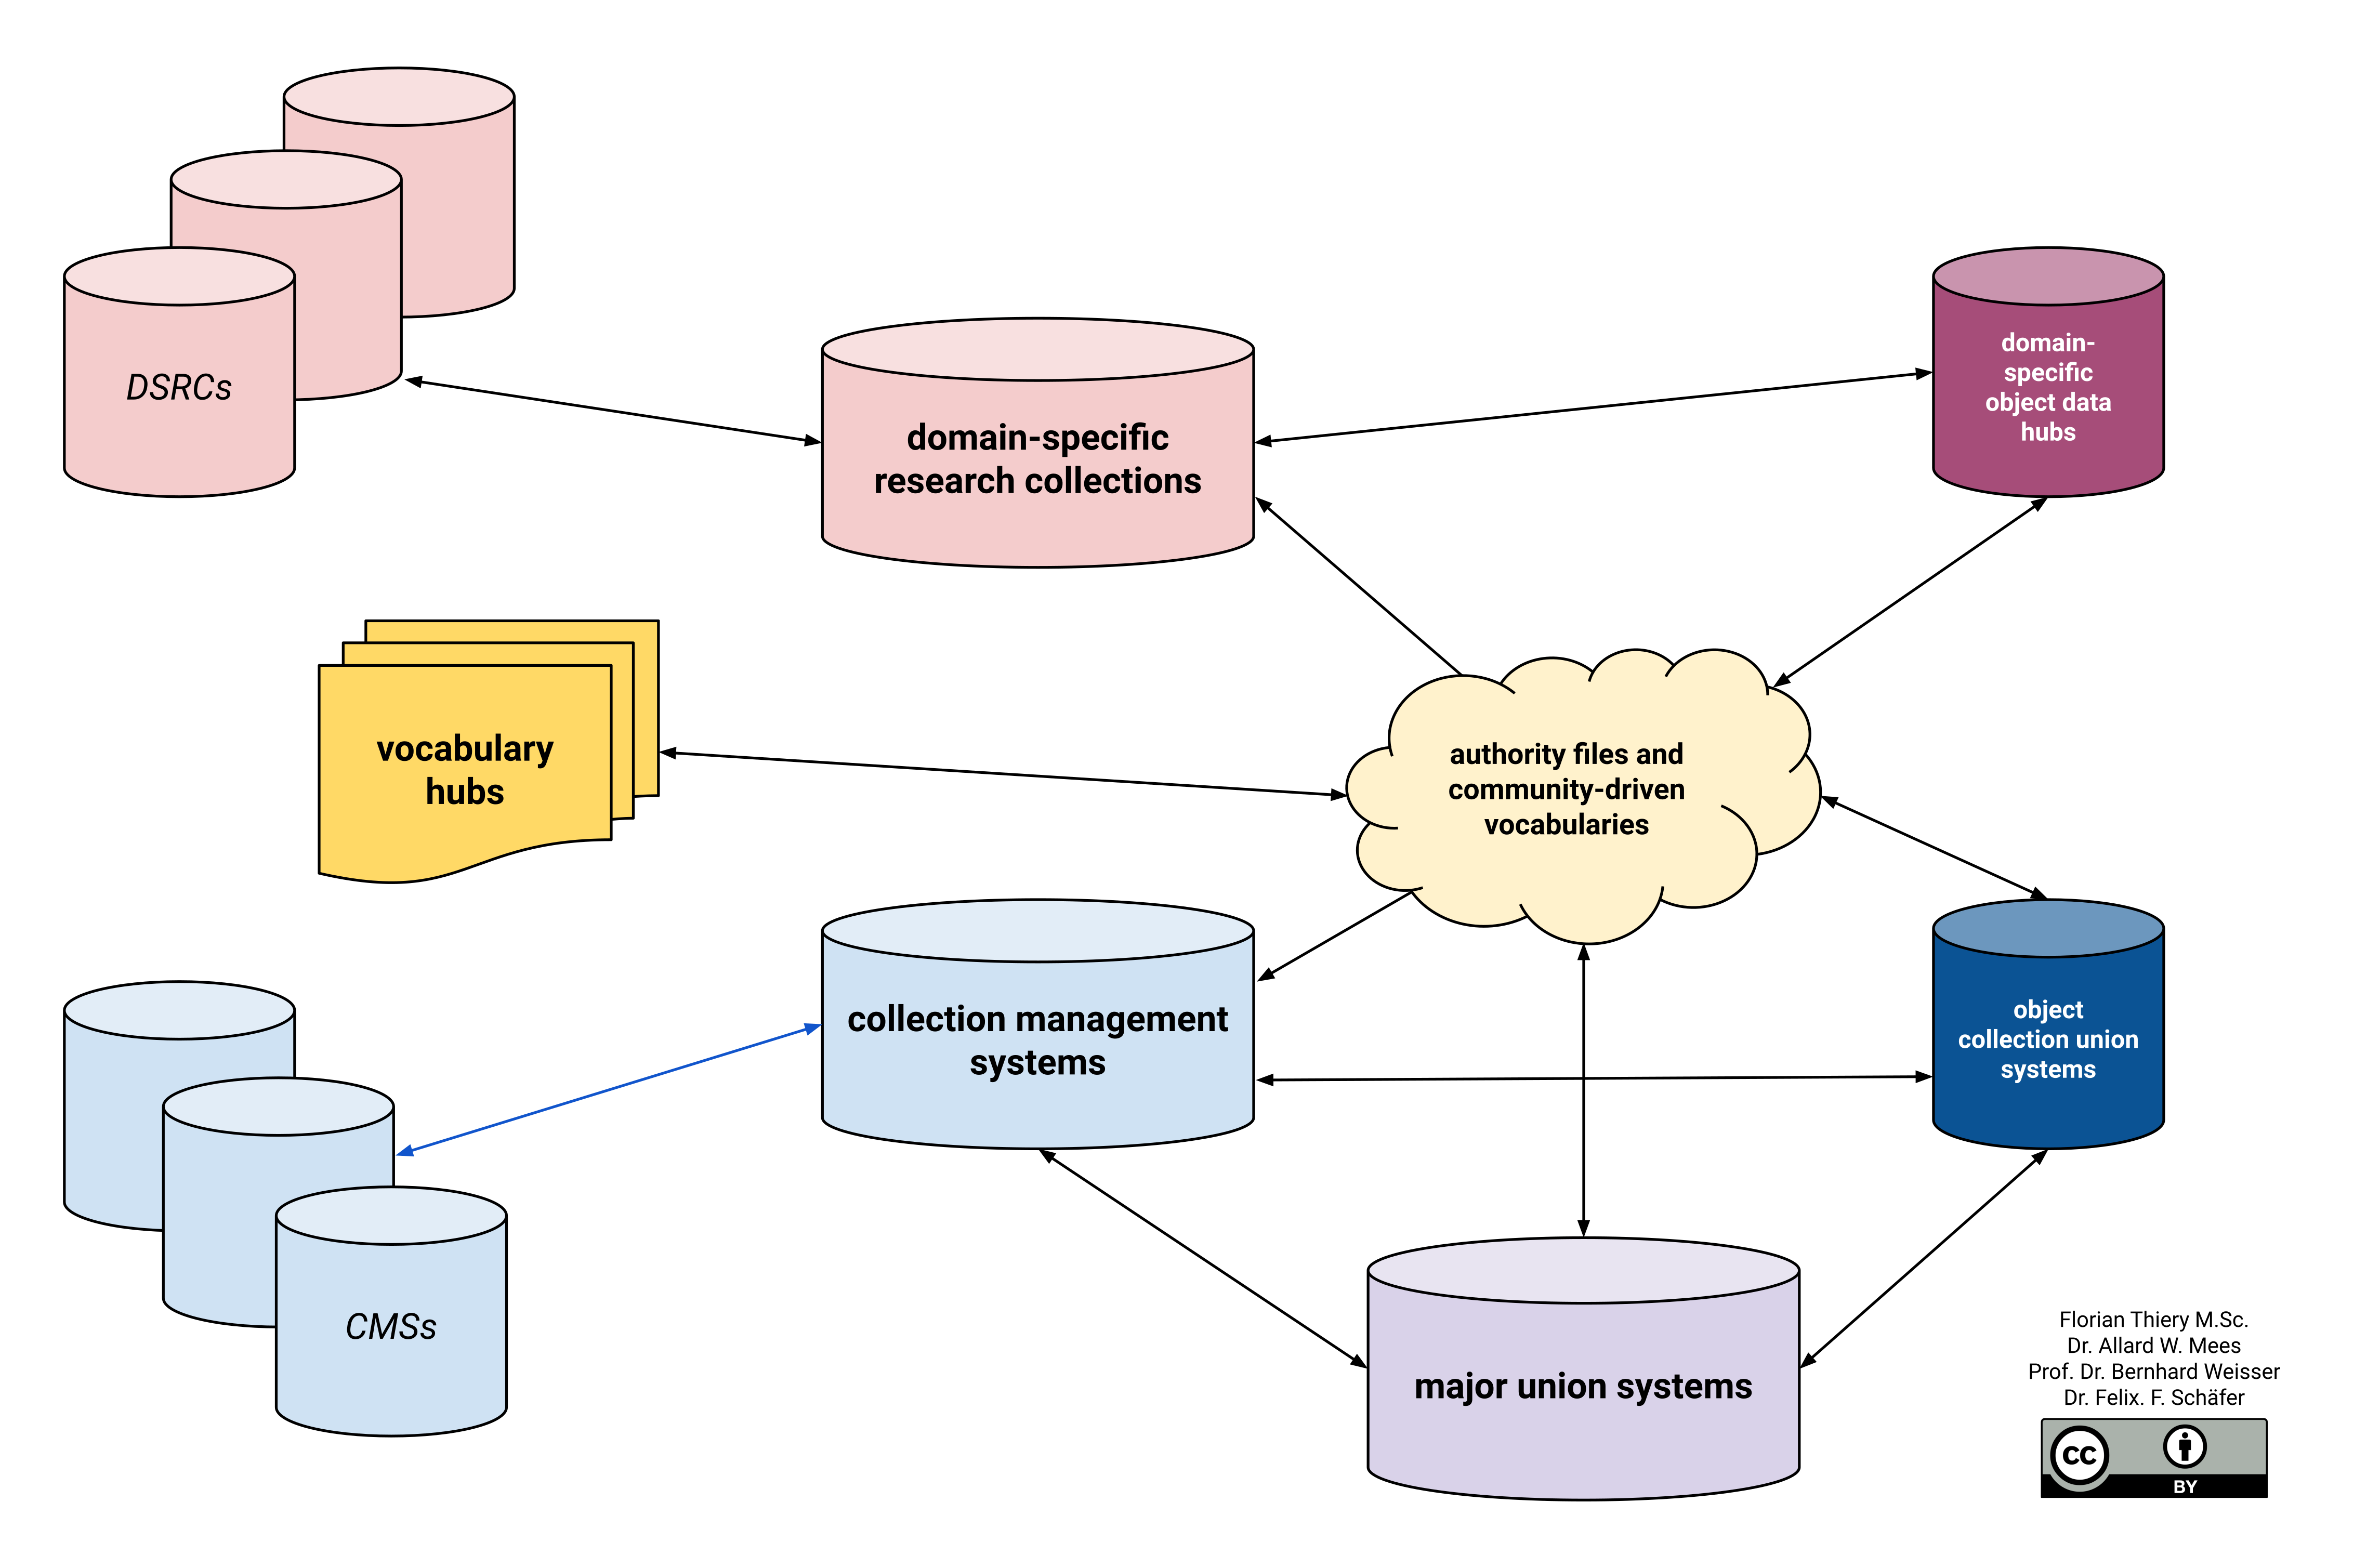
\includegraphics[scale=0.6]{img/Collection_Research_Network.png}
  \caption{Interaktion von Collection Research Systems im Sinne des FDM. [Florian Thiery, Allard W. Mees, Bernhard Weisser, Felix F. Schäfer, CC BY 4.0, via \href{https://commons.wikimedia.org/wiki/File:Collection_Research_Network.png}{Wikimedia Commons}]}
  \label{fig:network}
 \end{center}
\end{figure}

\begin{sidewaysfigure}[ht]
 \begin{center}
  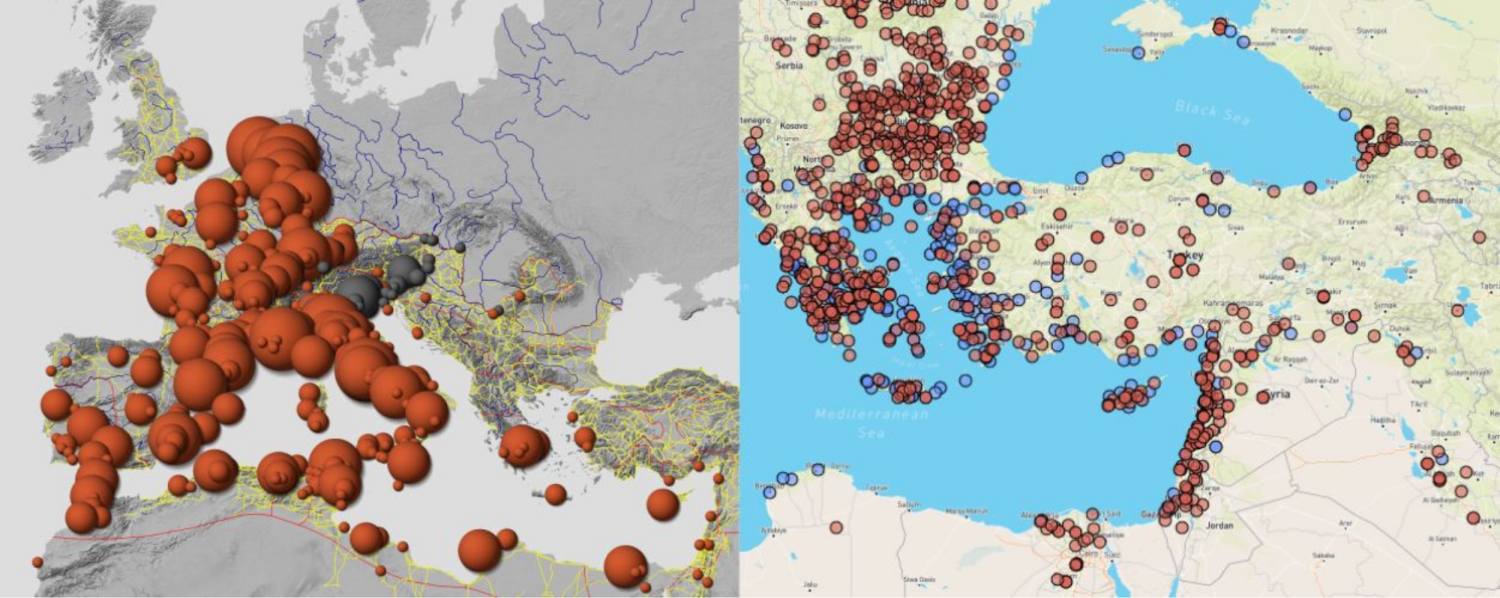
\includegraphics[scale=0.75]{img/map.pdf}
  \caption{Links: Verbreitung von Dressel 6b-Amphoren (schwarz) und Terra Sigillata (orange) aus Pisa; rechts: Münzstätten (blau) und Fundorte von Münzen aus Silber (rot). Die Karten zeigen Daten, die aus verschiedenen dezentralen Datenbanken über die jeweiligen  maschinenlesbaren Schnittstellen abgefragt wurden. [Daten-Quellen: links: \url{https://rgzm.github.io/samian-lod} und \url{https://romanopendata.eu}; rechts: \url{http://coinhoards.org}; Bild-Quellen: links: Samian Research, rechts: CoinHoards]}
  \label{fig:map}
 \end{center}
\end{sidewaysfigure}

\bigskip
\end{document}